\paragraph{Sơ đồ tuần tự luồng Yêu cầu Khôi phục Mật khẩu (Forgot Password / Recovery)}

Luồng nghiệp vụ này mô tả
quy trình người dùng gửi
yêu cầu khôi phục mật khẩu
thông qua địa chỉ email đăng ký
để nhận liên kết xác nhận từ Auth Service.

\begin{figure}[H]
\centering
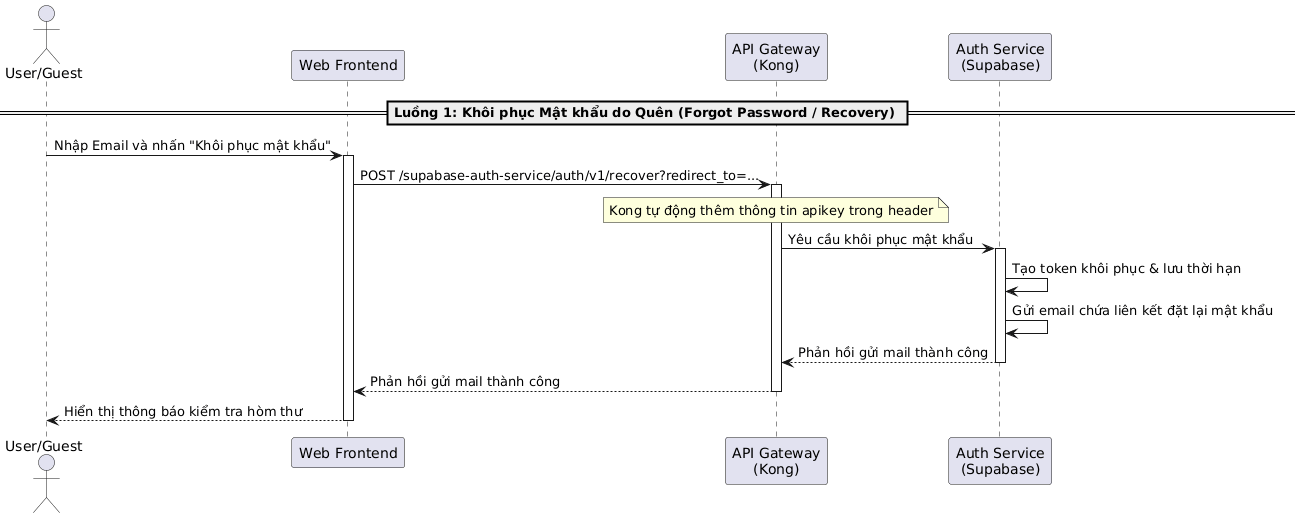
\includegraphics[scale = 0.2]{contents/Sequence/UML-Sequence-UserForgotPasswordRequest.png}
\caption{Sơ đồ tuần tự luồng Yêu cầu Khôi phục Mật khẩu}
\end{figure}

\subparagraph{Các thành phần tham gia}

\begin{table}[H]
\centering
\renewcommand{\arraystretch}{1.3}

\begin{tabular}{|l|l|p{5cm}|}
\hline
\textbf{Thành phần} & \textbf{Phân loại} & \textbf{Vai trò trong hệ thống} \\ \hline
User/Guest & Actor & Người dùng hoặc khách yêu cầu khôi phục mật khẩu. \\ \hline
Web Frontend & Component & Giao diện web Next.js. \\ \hline %%%% Component & Giao diện Next.js thu nhận email và gửi yêu cầu. \\ \hline
API Gateway (Kong) & Component & Cổng API chuyển tiếp các yêu cầu API. \\ \hline %%%% Component & Định tuyến yêu cầu phục hồi tài khoản tới Auth Service. \\ \hline
Auth Service (Supabase) & Microservice & Dịch vụ Supabase Auth thực hiện xác thực, quản lý token khôi phục và gửi email khôi phục mật khẩu. \\ \hline
\end{tabular}
\caption{Các thành phần tham gia luồng Yêu cầu Khôi phục Mật khẩu}
\end{table}

\subparagraph{Mô tả tổng quan}

\begin{itemize}
\item Người dùng điền Email và nhấn khôi phục. Frontend gửi yêu cầu \texttt{POST /supabase-auth-service/auth/v1/recover} qua Kong đến Auth Service.
\item Auth Service tự tạo token khôi phục, lưu thời hạn sử dụng và trực tiếp gửi email chứa liên kết đặt lại mật khẩu tới người dùng.
\end{itemize}
